\documentclass[10pt,twocolumn,a4paper]{article}

\usepackage[margin=2cm,columnsep=0.8cm]{geometry}
\usepackage[T1]{fontenc}
\usepackage[utf8]{inputenc}
\usepackage{mathptmx}
\usepackage{microtype}
\usepackage{amsmath,amssymb}
\usepackage{booktabs}
\usepackage{array}
\usepackage{graphicx}
\usepackage{xcolor}
\usepackage{tikz}
\usetikzlibrary{arrows.meta,positioning,calc}
\usepackage{pgfplots}
\pgfplotsset{compat=1.16}
\usepackage[font=small,labelfont=bf,labelsep=period]{caption}
\usepackage{enumitem}
\usepackage[numbers,sort&compress]{natbib}
\usepackage[colorlinks=true,linkcolor=blue!50!black,citecolor=blue!50!black,urlcolor=blue!50!black]{hyperref}

\renewcommand{\thesection}{\Roman{section}}
\renewcommand{\thesubsection}{\thesection.\Alph{subsection}}
\setlist{nosep,leftmargin=*}
\setlength{\parskip}{0pt}
\setlength{\parindent}{1em}
\renewcommand{\arraystretch}{1.1}
\bibpunct{[}{]}{,}{n}{}{,}

\newcommand{\Gthree}{G3}
\newcommand{\Gtwo}{G2}
\newcommand{\Gone}{G1}

\title{\textbf{Predictive Modelling of Student Grades and\\Deterministic Target-Score Estimation}}

\author{
  \begin{tabular}[t]{c@{\hspace{2.5cm}}c}
    \textbf{Dauren Shatyrbekov} & \textbf{Sanzhar Omarov}\\
    {\small 242462@astanait.edu.kz} & {\small 241325@astanait.edu.kz}
  \end{tabular}\\[4pt]
  Astana IT University, Astana, Kazakhstan\\
  Group BDA-2405 \quad|\quad Research Methods, Final Paper
}
\date{}

\begin{document}

\twocolumn[
\begin{@twocolumnfalse}
\maketitle
\vspace{-1.2em}
\begin{abstract}
\noindent During a semester, students usually ask two questions: what final grade can I get, and what score do I need to reach my target grade? This paper explains that these two questions need two different methods. The required score is an exact calculation when the current marks and the assessment weights are known. The final grade is not known in advance, so it must be estimated. In this research we built a required-score calculator and compared four regression models (Linear Regression, Support Vector Regression, Random Forest and Gradient Boosting) with two simple baselines. We used the public UCI Student Performance dataset with 1,044 student-course records, and the models predict the final grade G3 after the second grading period. The G2-only baseline had the lowest MAE (0.847), but Random Forest had the lowest RMSE (1.634) and the highest $R^2$ (0.827). Five-fold cross-validation gave a Random Forest MAE of $0.874 \pm 0.070$. The calculator passed all validation tests. Our main conclusion is that the second-period grade carries most of the useful information, and that an exact required score should always be shown separately from a forecast.
\end{abstract}
\noindent\textbf{\textit{Index Terms}---}student grade prediction, required score, educational data mining, regression, Random Forest, learning analytics
\vspace{1.2em}
\end{@twocolumnfalse}
]

%==============================================================
\section{Introduction}
%==============================================================
Student performance is an important topic in higher education. Universities collect many types of information about students, for example grades, attendance and activity in online learning systems. This information can help researchers to understand student performance and to find learning problems early. This direction is part of educational data mining and learning analytics \cite{baker2009,siemens2011,romero2020}.

In most university courses the final grade is made from several assessments, such as quizzes, a midterm exam, projects and a final exam. Every assessment has its own weight, and all weights together are equal to 100\%. During the semester a student already knows some marks, but the other marks are still unknown. Because of this, a student can ask two different questions. First, what final grade can I expect? Second, what score do I need on the remaining work to reach my target grade?

In our opinion, these two questions are often mixed, but they are not the same. The second question has an exact answer when the marks and the weights are correct, because it is only a formula. The first question does not have an exact answer, because the final grade depends on future results. Machine learning can give an estimate, and since grades are numbers, regression models are a natural choice \cite{breiman2001,pedregosa2011}. The problem starts when a student reads a predicted grade as a promise. If a model says 15 out of 20, the real result can be different, and a student who plans study time using this number can make a wrong decision.

This paper and the research behind it try to keep the two answers separate. We built a required-score calculator and, in parallel, a grade prediction experiment on real student data. The prediction part answers how good an estimate can be, and the calculator part answers what is needed exactly. We think that students get a more honest picture when they see both answers with their different level of certainty.

\subsection{Research Questions and Hypotheses}
The research is guided by three research questions:
\begin{itemize}
  \item \textbf{RQ1:} How accurately can earlier grades and student features estimate the final grade \Gthree?
  \item \textbf{RQ2:} Which baseline or regression model gives the lowest test error?
  \item \textbf{RQ3:} Can the required-score calculator return correct results for valid inputs?
\end{itemize}
Two hypotheses were also defined in the earlier stage of the research. \textbf{H1:} the calculator error will be zero, except for small rounding differences. \textbf{H2:} Random Forest and Gradient Boosting will have lower MAE and RMSE than Linear Regression.

\subsection{Contributions}
This paper has four contributions.
\begin{enumerate}
  \item It separates the exact score calculation from the estimated final grade prediction.
  \item It compares four regression models and two baselines on the same real dataset and the same test set.
  \item It checks the calculator with test cases whose answers are known in advance.
  \item It shows with real numbers that the simple G2-only rule is very hard to beat, and it discusses why.
\end{enumerate}

\subsection{How This Research Developed}
This paper combines the work from all the tasks of the course. In Assignment~1 we reviewed ten technical studies and ten review papers about student performance prediction, and from them we found a research gap. In Assignment~2 we described the methods and materials: the calculator formulas, the possible data sources and the evaluation metrics. The midterm poster turned this into a research proposal, and at that time we had no empirical results. In Assignment~4 we wrote a full paper in which the calculator was tested on 550 generated scenarios. However, the model comparison in that paper used simulated values only, and they were not measurements from real students. For this reason, \emph{those simulated values are not used as evidence anywhere in this paper}. Finally, for the endterm presentation and the final poster we trained the models on a real public dataset, and all numbers reported in the results section come from these executed experiments.

\subsection{Structure of the Paper}
Section~II reviews the related work and the research gap. Section~III describes the methods and materials. Section~IV presents the results. Section~V discusses the results and the limits of the research. Section~VI gives the conclusion and future work.

%==============================================================
\section{Literature Review}
%==============================================================
\subsection{Educational Data Mining and Learning Analytics}
Educational data mining and learning analytics use student data to understand learning and to support decisions of teachers and students \cite{baker2009,siemens2011,romero2020}. Student performance prediction is one of the most common tasks in this area. We reviewed ten systematic reviews and overview papers on this topic \cite{namoun2021,zhang2021,sekeroglu2021,balaji2021,roslan2022,alalawi2023,alwarthan2022,chaka2022,almalawi2024,chen2025}. From them we understood that the usual approach is supervised learning, where the inputs are grades, academic history or learning activity, and the output is a grade or a performance category.

\subsection{Technical Studies by Input and Purpose}
Instead of describing every paper one by one, we grouped ten technical studies by their inputs and purpose (Table~\ref{tab:lit}). We think this is more useful, because it shows what each group can and cannot do for our problem.

\begin{table*}[t]
\centering
\caption{Grouping of the technical studies reviewed in Assignment~1.}
\label{tab:lit}
\small
\begin{tabular}{p{2.7cm}p{3.9cm}p{4.3cm}p{3.9cm}}
\toprule
\textbf{Approach / data} & \textbf{Main idea} & \textbf{Limitation for our problem} & \textbf{Sources}\\
\midrule
Regression on partial grades & Early partial grades can give a useful final-grade estimate with SVR and ensembles & It predicts an outcome, not the required score & \cite{hidalgo2023}\\
Random Forest and academic history & Prior grades and predictor importance help to make forecasts & Historical inputs may not be available & \cite{musso2020,yagci2022,nachouki2023,alamgir2024,wang2022}\\
AI and online learning data & Learning activity and non-personal inputs can support prediction & Context and feature availability are different in each case & \cite{jiao2022,chavez2023}\\
Classification of academic records & Classifiers compare categories of performance & Categories do not solve weighted target scores & \cite{ahmed2024,khairy2024}\\
\bottomrule
\end{tabular}
\end{table*}

Three of these studies are the closest to our research. The first one predicts the final grade from partial course grades with a regression model \cite{hidalgo2023}. The second one uses Random Forest and focuses on which predictors are important \cite{nachouki2023}. The third one tries to predict performance without personal information \cite{chavez2023}. Other work looked at public datasets and at early prediction from learning management system logs \cite{kuzilek2017,balcioglu2025,ng2021,badal2023,santos2023}, and at hybrid machine learning methods \cite{arashpour2023}. The dataset that we selected for our experiment was introduced in \cite{cortez2008}. According to our reading, the authors of that paper found that earlier period grades make prediction better and that tree-based methods work well.

\subsection{Reported Problems}
The reviews report several repeated problems: weak data quality, inconsistent validation, different definitions of the outcome, and poor comparability between studies \cite{namoun2021,sekeroglu2021,roslan2022,alwarthan2022,chaka2022,hellas2018}. This means that the accuracy numbers from two papers cannot be compared directly if the datasets, the features and the evaluation methods are different. Another important problem is data leakage. A model can look much better than it really is if it uses information that will not be available at the real prediction time \cite{kaufman2012}. We kept this problem in mind when we designed the experiment.

\subsection{Research Gap}
In the work that we reviewed, forecasting is the main topic. The exact score that a student still needs, when the weights are known, receives much less attention. We want to be careful here: this is a gap inside the literature that we reviewed, and we do not claim that grade calculators do not exist. Our research tries to fill this gap by keeping the exact calculation independent from the uncertainty of machine learning.

%==============================================================
\section{Methods and Materials}
%==============================================================
\subsection{Research Design}
The research is quantitative \cite{creswell2018}. Numbers are used in all parts: the grades, the calculation errors and the prediction metrics. The system has two components with different inputs, outputs and evaluation rules (Fig.~\ref{fig:workflow}).

\begin{figure}[t]
\centering
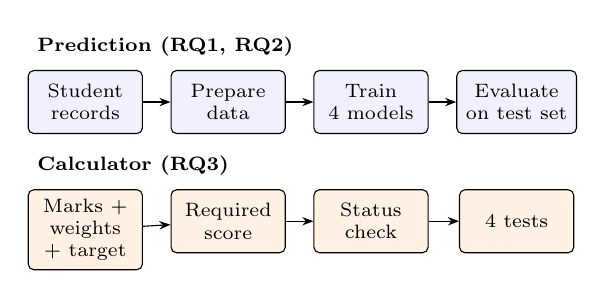
\begin{tikzpicture}[
  node distance=0.35cm,
  box/.style={draw,rounded corners=2pt,align=center,font=\scriptsize,minimum height=0.8cm,minimum width=1.45cm,fill=blue!6},
  box2/.style={draw,rounded corners=2pt,align=center,font=\scriptsize,minimum height=0.8cm,minimum width=1.45cm,fill=orange!10},
  arr/.style={-{Stealth[length=4pt]}}]
  \node[box] (a1) {Student\\records};
  \node[box,right=of a1] (a2) {Prepare\\data};
  \node[box,right=of a2] (a3) {Train\\4 models};
  \node[box,right=of a3] (a4) {Evaluate\\on test set};
  \draw[arr] (a1)--(a2); \draw[arr] (a2)--(a3); \draw[arr] (a3)--(a4);
  \node[box2,below=0.7cm of a1] (b1) {Marks +\\weights\\+ target};
  \node[box2,below=0.7cm of a2] (b2) {Required\\score};
  \node[box2,below=0.7cm of a3] (b3) {Status\\check};
  \node[box2,below=0.7cm of a4] (b4) {4 tests};
  \draw[arr] (b1)--(b2); \draw[arr] (b2)--(b3); \draw[arr] (b3)--(b4);
  \node[font=\scriptsize\bfseries,anchor=south west] at ($(a1.north west)+(0,0.05)$) {Prediction (RQ1, RQ2)};
  \node[font=\scriptsize\bfseries,anchor=south west] at ($(b1.north west)+(0,0.05)$) {Calculator (RQ3)};
\end{tikzpicture}
\caption{Workflow of the research. Top: grade prediction. Bottom: required-score calculator.}
\label{fig:workflow}
\end{figure}

The prediction is a statistical estimate, and the calculation is a deterministic result under the given weights. We evaluate them separately, because they have different purposes.

\subsection{Required-Score Calculator}
Every assessment $i$ has a score $s_i$ and a weight $w_i$, and the weights must add up to 1. The final grade is
\begin{equation}
G_{final}=\sum_{i=1}^{n}s_i w_i .
\end{equation}
If some assessments are completed (the set $C$), their contribution is already known. For a target grade $T$, the remaining amount is
\begin{equation}
R = T-\sum_{i\in C}s_i w_i .
\end{equation}
When the remaining assessments have the total weight $w_r$, the required score is
\begin{equation}
S_{req}=\frac{R}{w_r}=\frac{T-\sum_i s_i w_i}{w_r}.
\end{equation}
The calculator returns a status together with the number:
\begin{itemize}
  \item \textit{feasible}, if $0 < S_{req} \le S_{max}$;
  \item \textit{already reached}, if $S_{req} \le 0$, because the completed marks are enough;
  \item \textit{impossible}, if $S_{req} > S_{max}$, where $S_{max}$ is the maximum score (20 in the final experiment);
  \item \textit{rejected}, if the weights or the scores are not valid, for example if the weights do not add up to 1.
\end{itemize}
An impossible target should never be shown as a normal answer. We think this is important for students, because a required score above the maximum is not the same as a ``low chance''. It simply cannot be reached under the grading scheme.

When more than one assessment remains, the same score can be assumed for all remaining work, or several combinations can be shown. For example, suppose a course has five assessments with weights 0.10, 0.10, 0.30 (midterm), 0.10 and 0.40 (final exam), and a student has $80$, $70$ and $75$ on the first three. The known contribution is $37.5$, and the student wants a final grade of $75$ on a 0--100 scale. Table~\ref{tab:alt} shows that the required score on the fourth assessment changes when the final exam result changes. This example is only an illustration of the calculation, not an empirical result.

\begin{table}[t]
\centering
\caption{Illustrative alternatives for two remaining assessments (target 75, known contribution 37.5; scale 0--100).}
\label{tab:alt}
\small
\begin{tabular}{ccc}
\toprule
\textbf{Final exam} & \textbf{Required on 4th} & \textbf{Status}\\
\midrule
60 & 135 & Impossible\\
70 & 95 & Feasible\\
80 & 55 & Feasible\\
\bottomrule
\end{tabular}
\end{table}

To check the calculator, the system answer is compared with a reference answer that is calculated manually or with exact arithmetic:
\begin{equation}
E_{calc}=\left|G_{system}-G_{reference}\right| .
\end{equation}
If the calculator is correct, this error must be zero, and only a very small rounding difference is allowed. For different score combinations, the scenario error is
\begin{equation}
E_{scenario}=\left|T-\sum_{i=1}^{n}s_i w_i\right| ,
\end{equation}
and it should also be close to zero.

\subsection{Dataset}
For the prediction part we used the public UCI Student Performance dataset (UCI Machine Learning Repository, Dataset~320) \cite{cortez2008}. The data come from two Portuguese secondary schools and cover two subjects: mathematics and Portuguese language. The dataset has 1,044 student-course records, where 395 records are for mathematics and 649 records are for Portuguese. After we added a course label, the table has 34 columns: 33 input features and one target. The target is \Gthree, the final grade on a 0--20 scale. The inputs include the earlier grades \Gone{} and \Gtwo, the number of absences, study time, and personal and school context such as age, sex, parents' education, family support, free time and alcohol use. No missing values were detected. The mean of \Gthree{} is 11.34, the median is 11, and the range is from 0 to 20.

We selected a public dataset because real student records are not easy to access, and public data can be used for testing without personal information problems. We also know that this dataset does not represent our university, and we discuss this limit in Section~V.

\subsection{Data Preprocessing}
The same preparation pipeline was applied to the training and test data. The steps were:
\begin{itemize}
  \item check data types, value ranges, missing values and duplicates;
  \item separate \Gthree{} as the target and keep \Gone{} and \Gtwo{} as earlier grades;
  \item one-hot encode 18 categorical inputs and scale 15 numeric inputs;
  \item use median and mode imputation inside the pipeline as a safety step;
  \item fix the random seed to 42 and make an 80/20 split, which gives 835 training rows and 209 test rows.
\end{itemize}
All encoding and scaling steps were fitted inside the training pipeline only. This is important, because it avoids leakage from the test data into the training process \cite{kaufman2012}. The forecast is made after the second grading period and before \Gthree{} is known, so \Gone{} and \Gtwo{} are available at prediction time.

\subsection{Models and Baselines}
Four regression models were trained: Linear Regression, Support Vector Regression (SVR) with an RBF kernel, Random Forest \cite{breiman2001} and Gradient Boosting \cite{friedman2001}. We chose them because each one has a different way to learn: a simple linear form, a kernel method, an ensemble of independent trees, and an ensemble of trees built one after another \cite{hastie2009}. Their settings are in Table~\ref{tab:settings}. The settings were fixed and not tuned.

\begin{table}[t]
\centering
\caption{Model settings (fixed, not tuned).}
\label{tab:settings}
\small
\begin{tabular}{lp{4.9cm}}
\toprule
\textbf{Model} & \textbf{Settings}\\
\midrule
Linear Regression & default\\
SVR & RBF kernel, $C=10$, $\varepsilon=0.5$\\
Random Forest & 400 trees, minimum leaf size 2\\
Gradient Boosting & 200 trees, learning rate 0.04, depth 2, Huber loss\\
\bottomrule
\end{tabular}
\end{table}

Two simple baselines were added. The \emph{mean baseline} predicts the average training grade for every test record, so it gives a floor for the error. The \emph{G2-only baseline} uses the second-period grade directly as the estimate of the final grade. This second baseline tests an important question: does a complex model give anything more than the latest grade? In Assignment~2 and in the midterm poster we planned to compare Random Forest and SVR with a mean baseline and a linear regression baseline. The G2-only baseline was added later, and it turned out to be a much stronger competitor.

\subsection{Evaluation Methods}
All models were evaluated on the same 209-record test set. Three metrics were used, where $y_i$ is the real grade, $\hat{y}_i$ is the predicted grade and $N$ is the number of test records:
\begin{align}
MAE &= \frac{1}{N}\sum_{i=1}^{N}\left|y_i-\hat{y}_i\right|,\\
RMSE &= \sqrt{\frac{1}{N}\sum_{i=1}^{N}\left(y_i-\hat{y}_i\right)^2}.
\end{align}
MAE is the average absolute error. RMSE punishes large errors more strongly. For both of them lower is better. The third metric, $R^2$, shows the share of the variation of the target that the model explains, and higher is better.

To check how much the result depends on one split, we also made a five-fold cross-validation for Random Forest (250 trees). To see which features are used by the model, we calculated permutation importance for Random Forest with 8 repeats, scored by MAE. This value is the increase in error when one feature is shuffled. It shows association with model performance, and it does not prove a cause. The calculator is a rule and not a model, so it is not checked by error metrics but by test cases.

\subsection{Tools, Reproducibility and Privacy}
We used Python with scikit-learn \cite{pedregosa2011}, and the code was run in Google Colab. The fixed seed, the documented preparation steps and the same test set for all models make the experiment repeatable. About privacy, the dataset is public and anonymised, and we did not collect any personal data. The calculator also does not need a student name or other personal details. This agrees with earlier work that tried to predict performance without personal information \cite{chavez2023}.

%==============================================================
\section{Results}
%==============================================================
\subsection{Calculator Validation (RQ3, H1)}
We start with a worked example from the final experiment. The target grade is 15 out of 20. The student has two completed marks: 14 with weight 0.30, and 16 with weight 0.40. The current contribution is $14\times0.30 + 16\times0.40 = 4.20+6.40=10.60$. The remaining weight is 0.30, so
\begin{equation}
S_{req}=\frac{15-10.60}{0.30}=14.67 .
\end{equation}
The student needs 14.67 out of 20 on the remaining assessment.

Table~\ref{tab:calc} shows the four test cases of the final experiment. In all cases the calculator output was the same as the expected result, so 4 of 4 tests passed. The calculator also showed the correct status for a target that was already reached (raw value $-2.00$), for an impossible target (required 47.0 out of 20), and it rejected the invalid weights.

\begin{table}[t]
\centering
\caption{Calculator tests in the final experiment (weights 0.30 and 0.40; remaining weight 0.30; scale 0--20).}
\label{tab:calc}
\small
\begin{tabular}{llccc}
\toprule
\textbf{Case} & \textbf{Marks} & \textbf{Target} & \textbf{Expected} & \textbf{Result}\\
\midrule
Feasible & 14, 16 & 15 & 14.67 & 14.67 \checkmark\\
Reached & 18, 18 & 12 & $\le 0$ & $-2.00$ \checkmark\\
Impossible & 5, 6 & 18 & 47.0 & 47.0 \checkmark\\
Bad weights & 14 & 15 & rejected & rejected \checkmark\\
\bottomrule
\end{tabular}
\end{table}

Before this, in Assignment~4, we also tested the calculator on a larger set of generated scenarios (scale 0--100), and each answer was compared with an independent reference calculated in exact rational arithmetic. Table~\ref{tab:calc550} shows that all 550 scenarios were handled correctly. For the 400 scenarios with a numerical answer, the largest error was 0.005 points, which is consistent with rounding to two decimal places. The other 150 scenarios gave a status message and not an ordinary number, as expected.

\begin{table}[t]
\centering
\caption{Calculator tests on generated scenarios (Assignment~4, scale 0--100).}
\label{tab:calc550}
\small
\begin{tabular}{lccc}
\toprule
\textbf{Scenario type} & \textbf{Tests} & \textbf{Correct} & \textbf{Max $E_{calc}$}\\
\midrule
One assessment left & 200 & 200 & 0.005\\
Several assessments left & 200 & 200 & 0.005\\
Target already reached & 50 & 50 & 0\\
Target above maximum & 50 & 50 & --\\
Weights not equal to 100\% & 50 & 50 & --\\
\midrule
Total & 550 & 550 & 0.005\\
\bottomrule
\end{tabular}
\end{table}

These results support H1 and give a positive answer to RQ3: for the valid inputs that we tested, the calculator returns correct results. We want to say clearly that this does not prove the calculator for every possible grading scheme. It only shows that the formula and the status rules were implemented correctly for the tested cases.

\subsection{Model Comparison (RQ1, RQ2, H2)}
Table~\ref{tab:models} shows the test-set metrics of all models and baselines, and Fig.~\ref{fig:errors} shows the errors in a chart. The G2-only baseline has the lowest MAE (0.847). Gradient Boosting is second by MAE (0.887) and has almost the same RMSE and $R^2$ as the G2 baseline. Random Forest has a higher MAE (0.924), but it has the lowest RMSE (1.634) and the highest $R^2$ (0.827). Linear Regression and SVR are weaker, and the mean baseline is far behind, with MAE 2.939 and a negative $R^2$.

\begin{table}[t]
\centering
\caption{Test-set metrics on 209 records (grades on a 0--20 scale).}
\label{tab:models}
\small
\begin{tabular}{lccc}
\toprule
\textbf{Model} & \textbf{MAE} & \textbf{RMSE} & \textbf{$R^2$}\\
\midrule
G2 baseline & \textbf{0.847} & 1.740 & 0.804\\
Gradient Boosting & 0.887 & 1.743 & 0.804\\
Random Forest & 0.924 & \textbf{1.634} & \textbf{0.827}\\
Linear Regression & 1.017 & 1.760 & 0.800\\
SVR & 1.130 & 1.896 & 0.767\\
Mean baseline & 2.939 & 3.948 & $-0.008$\\
\bottomrule
\end{tabular}
\end{table}

\begin{figure}[t]
\centering
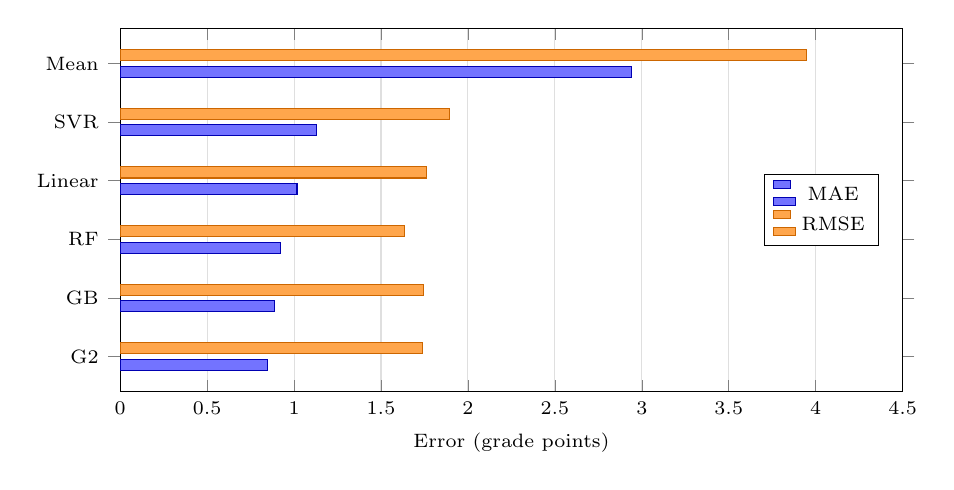
\begin{tikzpicture}
\begin{axis}[
  xbar,
  width=0.95\columnwidth,
  height=6.2cm,
  bar width=4pt,
  xmin=0, xmax=4.5,
  xlabel={Error (grade points)},
  symbolic y coords={Mean,SVR,Linear,RF,GB,G2},
  ytick=data,
  y dir=reverse,
  enlarge y limits=0.12,
  legend style={at={(0.97,0.5)},anchor=east,font=\scriptsize},
  tick label style={font=\scriptsize},
  label style={font=\scriptsize},
  xmajorgrids=true,
  grid style={gray!25}
]
\addplot[fill=blue!55,draw=blue!70!black] coordinates {(2.939,Mean) (1.130,SVR) (1.017,Linear) (0.924,RF) (0.887,GB) (0.847,G2)};
\addplot[fill=orange!70,draw=orange!80!black] coordinates {(3.948,Mean) (1.896,SVR) (1.760,Linear) (1.634,RF) (1.743,GB) (1.740,G2)};
\legend{MAE,RMSE}
\end{axis}
\end{tikzpicture}
\caption{MAE and RMSE of each model on the test set (RF: Random Forest, GB: Gradient Boosting).}
\label{fig:errors}
\end{figure}

For RQ1, the three best approaches estimate \Gthree{} with an MAE between 0.85 and 0.92 grade points on the 0--20 scale. For RQ2, the answer depends on the metric: the G2-only baseline has the lowest MAE, and Random Forest has the lowest RMSE and highest $R^2$. About H2, both Random Forest and Gradient Boosting have lower MAE and RMSE than Linear Regression, so H2 is supported on this test split. Random Forest also reached the benchmark that we planned in the midterm proposal: lower MAE than the mean baseline and the linear baseline, and no worse RMSE. However, it did not beat the later G2-only rule on MAE.

\subsection{Cross-Validation}
The five-fold cross-validation of Random Forest gave an MAE of $0.874 \pm 0.070$ (mean $\pm$ standard deviation over the folds). This value is close to the test-set MAE of 0.924, so the result does not seem to depend only on one lucky split.

\subsection{Feature Importance}
Fig.~\ref{fig:imp} shows the top six features by permutation importance for Random Forest. The second-period grade \Gtwo{} dominates, with an increase in MAE of 2.846 when it is shuffled. Absences are second (0.202), and \Gone{} is third (0.029). The next features (course, age and father's education) have very small values.

\begin{figure}[t]
\centering
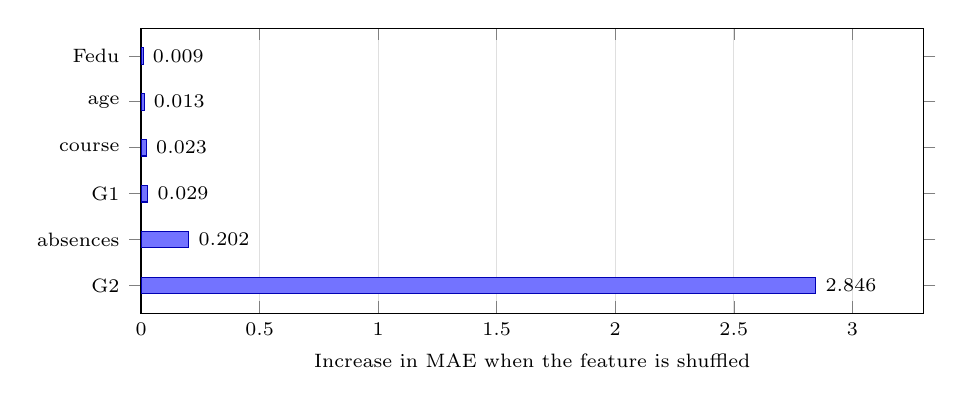
\begin{tikzpicture}
\begin{axis}[
  xbar,
  width=0.95\columnwidth,
  height=5.2cm,
  bar width=6pt,
  xmin=0, xmax=3.3,
  xlabel={Increase in MAE when the feature is shuffled},
  symbolic y coords={Fedu,age,course,G1,absences,G2},
  ytick=data,
  y dir=reverse,
  enlarge y limits=0.12,
  nodes near coords,
  nodes near coords align={horizontal},
  every node near coord/.append style={font=\scriptsize,/pgf/number format/fixed,/pgf/number format/precision=3},
  /pgf/number format/fixed,
  tick label style={font=\scriptsize},
  label style={font=\scriptsize},
  xmajorgrids=true,
  grid style={gray!25}
]
\addplot[fill=blue!55,draw=blue!70!black] coordinates {(0.009,Fedu) (0.013,age) (0.023,course) (0.029,G1) (0.202,absences) (2.846,G2)};
\end{axis}
\end{tikzpicture}
\caption{Random Forest permutation importance, top six features.}
\label{fig:imp}
\end{figure}

%==============================================================
\section{Discussion}
%==============================================================
\subsection{Meaning of the Results}
The two components of this research have a different nature. The calculator is a deterministic rule: the same input always gives the same output, and the answer can be checked by hand. The grade prediction is statistical, so its output is an estimate with an error. The results show this difference very clearly. The calculator was correct in all tests, but even the best predictors still have an average error of about 0.85--0.92 points. On a 0--20 scale this is not big, but it is enough to change a letter grade near a boundary. Because of this, we think that keeping the two answers separate is a good decision and not only a theoretical one.

\subsection{Why the G2 Baseline Is So Strong}
The most interesting result for us is that the simple G2-only rule has the lowest MAE, and that no model beat it on this metric. The permutation importance gives a similar message, because \Gtwo{} is much more important than any other feature. In our interpretation, this happens because the grades inside one course are connected: the second-period grade is already very close to the final grade, so the other 32 inputs add only a little new information. This agrees with the earlier result on the same dataset, where period grades improved prediction and Random Forest was among the best methods \cite{cortez2008}. It also agrees with the university study where prior performance was the leading predictor in a Random Forest model \cite{nachouki2023}. The practical lesson for us is that a complex model should always be compared with a simple baseline, otherwise the benefit of the complexity can be overestimated.

At the same time, the differences between the top models are small. The gap between the G2 baseline and Random Forest in MAE is about 0.08 points, which is similar in size to the standard deviation of 0.070 between cross-validation folds. We have only 209 test records and we did not calculate confidence intervals, so we do not want to claim that one of the top three approaches is clearly the best. A formal comparison with confidence intervals, as discussed in our earlier work, is a better next step.

\subsection{Random Forest, SVR and the Previous Literature}
Random Forest has a higher MAE than the G2 rule but the best RMSE and $R^2$. A possible explanation is that it avoids some large errors, for example when the final grade is near zero, but we did not test this, so it remains only an idea. Another result that we did not expect is that SVR was the weakest of the four models. One earlier study on partial course grades found SVR to be the best model \cite{hidalgo2023}. Our SVR was weak maybe because the data are different and because we used fixed untuned settings (Table~\ref{tab:settings}). This is also an example of the comparability problem from the literature \cite{hellas2018}: a ranking of models in one dataset should not be copied to another dataset.

\subsection{Link to Student Planning}
Our idea is that the two outputs support different student behaviour. A required score such as 14.67 out of 20 is a specific goal, and it is easy to follow it during the semester. Goal-setting theory says that specific and difficult goals help performance when the person gets feedback about progress \cite{locke2002}, and self-regulated learning stresses the monitoring of progress against such goals \cite{zimmerman2002}. A predicted grade is different, because it is a forecast and not a goal. Also, ``impossible'' is a different message from ``low chance'': the first one is a fact under the grading scheme, and the second one is a probability. We did not run a user study, so we cannot say that the calculator improves student results. This is only our interpretation of how the results can be used.

\subsection{Leakage and Prediction Time}
Data leakage means that the model uses information that is not available at the real prediction time \cite{kaufman2012}. In this research the forecast is made after the second grading period, so \Gone{} and \Gtwo{} are legal inputs. Still, this timing has a cost: the forecast is not an early warning from the start of the semester. In Assignment~4 we also planned to compare the errors with and without leakage columns, but we did not do this comparison on real data, so we cannot report any number about it. We only used leakage as a design rule for choosing the inputs.

\subsection{Limitations and Threats to Validity}
The conclusions of this paper describe this dataset and this setting only. The main limits are:
\begin{itemize}
  \item The data come from two Portuguese secondary schools, not from our university.
  \item The split was random and not grouped by student. A student can be in both courses, so the test scores may be optimistic.
  \item The forecast is made after period 2, not at the beginning of the semester.
  \item The model settings were fixed and not tuned, and only one test split and one cross-validation run were used.
  \item The calculator assumes linear weights. Rounding, minimum exam thresholds and resits are not encoded.
  \item Permutation importance shows association with the performance of the model, not a cause.
  \item No user study was made.
\end{itemize}

%==============================================================
\section{Conclusion and Future Work}
%==============================================================
This paper studied two tasks that students often mix: the exact calculation of the score needed for a target grade, and the estimation of the final grade with regression models. We used a real public dataset with 1,044 student-course records and compared four regression models with two baselines on the same test set.

The main findings are the following. The calculator passed all of its validation tests, so RQ3 has a positive answer. The final grade \Gthree{} was estimated with an MAE between 0.85 and 0.92 points on the 0--20 scale (RQ1). The G2-only baseline had the lowest MAE (0.847), and Random Forest had the lowest RMSE (1.634) and the highest $R^2$ (0.827) (RQ2). The five-fold MAE of Random Forest was $0.874\pm0.070$. The second-period grade was by far the most important feature. In our opinion, the contribution of this research is mainly in the clear separation of a forecast from an exact calculation, and in the honest comparison with a simple baseline.

For future work, we want to use authorised and anonymised local data from our university and to split the data by student. We also want to calculate confidence intervals, to study the prediction uncertainty, and to check the performance for different courses. A possible extension for the calculator is to add rounding rules, minimum exam thresholds and resits. Finally, a small user study can show whether students really make better plans when they see the required score together with a forecast.

%==============================================================
\bibliographystyle{ieeetr}
\bibliography{references}

\end{document}
